%!TEX program=xelatex
\documentclass[UTF-8, a4paper, 12pt]{ctexart}
\setlength{\parindent}{0pt}
\usepackage{setspace}
\renewcommand{\baselinestretch}{1.5}
\usepackage{tikz}
\usepackage{pgfplots}
\usepackage{textcomp}
\usepackage[left=2.50cm, right=2.50cm, top=2.50cm, bottom=2.50cm]{geometry}
\usepackage{fancyhdr}
\usepackage{enumerate}
\pagestyle{fancy}
\rhead{\center{\small{华南理工大学大学城校区物理实验报告}}}

\begin{document}
    \begin{center}
        \zihao{-2}\heiti{新能源的综合利用及探索 预习报告}
        

        \zihao{-4}\songti{2020级 \quad 计算机科学与技术(全英创新班)\quad 王樾}
    \end{center}
    \zihao{4}\heiti{引言:}\zihao{-4}
    \songti
    燃料电池是以氢和氧为原料通过电化学反应直接产生电力的装置,这种新型电池的效率高于燃烧燃料的热机。氢氧燃料电池的反应生成物为水,环保无污染,且氢的储能密度远高于其他电池。当前燃料电池的主要种类有碱性燃料电池、质子交换膜燃料电池、直接甲醇燃料电池、熔融碳酸盐燃料电池与固体氧化物燃料电池等基本类型。在未来,燃料电池将成为主要的清洁能源,而太阳能将作为主要的能源形式。

    \textbf{\zihao{4} \heiti{一、实验目的}}

    \zihao{-4}\songti

    \begin{enumerate}[(1)]
        \item 了解燃料电池的工作原理。
        \item 观察实验中的能源转换过程。
        \item 测量太阳能电池的输出特性。
    \end{enumerate}

    \textbf{\zihao{4} \heiti{二、实验仪器}}

    \zihao{-4}\songti

    太阳能电板、电阻箱。
    % TODO

    \textbf{\zihao{4} \heiti{三、实验原理}}

    \zihao{-4}\songti

    \begin{center}
        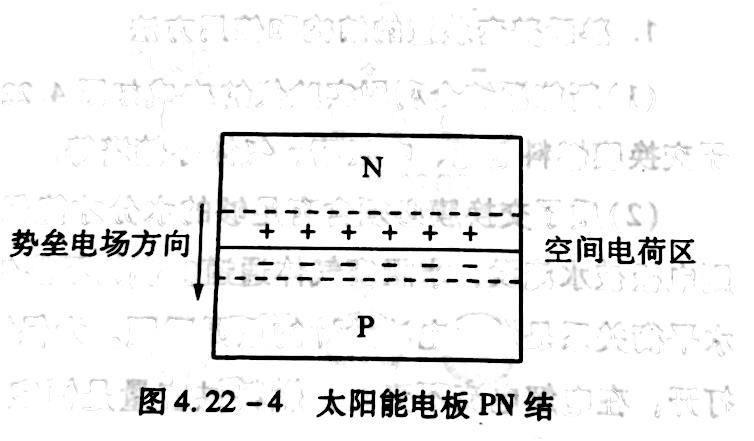
\includegraphics{4.22_1.jpg}
    \end{center}

    太阳能电池利用半导体PN结受光照射时的光伏效应发电。太阳能电池的基本结构就是一个大面积的PN结。

    P型半导体有很多空穴,却几乎没有自由电子;N型半导体有很多自由电子,却几乎没空穴。当两者结合形成PN结时,N型半导体的自由电子向P区扩散,P型半导体的空穴向N区扩散,在PN结附近形成了空间电荷区和势垒电场。在势垒电场的作用下,最终使得流过PN结的净电流为零。

    当电池受到光照时,部分电子被激发而产生了电子—空穴对,在PN结激发的电子和空穴分别被势垒电场推向N区和P区,使得N区有过量电子而带负电,P区有过量空穴而带正电,从而形成了光伏效应。此时如果将两端接入外电路,就可以向负载输出电能。

    在一定光照条件下,改变太阳能电池负载电阻的大小,测量出输出电压与电流的关系,则如图所示。

    \begin{center}
        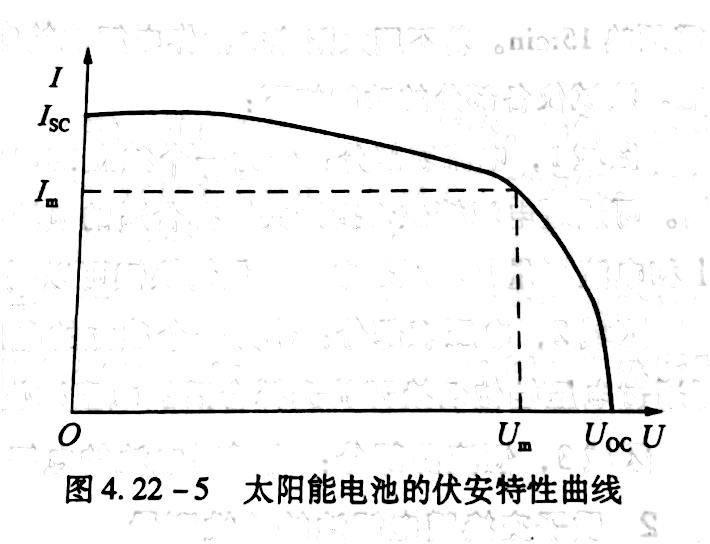
\includegraphics{4.22_2.jpg}
    \end{center}

    $U_{OC}$代表开路电压,$I_{SC}$代表短路电路,虚线围出的最大面积代表太阳能电池的最大输出功率,此时的电压记为$U_m$,电流记为$I_m$。

    定义填充因子$FF$为

    $$FF = \frac{U_m I_m}{U_{OC} I_{SC}}$$

    填充因子是评价太阳能电池输出电能能力好坏的重要参数,$FF$值越大,表明电池光电转换效率越高。

    \textbf{\zihao{4} \heiti{四、内容步骤}}

    \zihao{-4}\songti

    \begin{enumerate}[(1)]
        \item 按实验要求连接好装置,将电流测量端口与可变负载串联后接入太阳能电池的输出端。

        \item 将电压表并联到太阳能电池的两端。
        
        \item 保持光照不变,改变太阳能电池负载电阻的大小,测量相应电阻大小下,太阳能电池的输出电压值和输出电流值,并计算输出功率,记录于表。
    \end{enumerate}

\end{document}